\documentclass[12pt]{article}

\usepackage[utf8]{inputenc}
\usepackage[english, russian]{babel}

%\usepackage[T2A]{fontenc} 

\usepackage{slides}

\hyphenpenalty=5000
\tolerance=1000

% ШРИФТЫ
% Нужны рубленные шрифты -- раскомментируйте стоку ниже. 
% Нужны шрифты с засечками --- закомментируйте эту строку. 
\renewcommand{\familydefault}{\sfdefault} % Переключает на рубленный шрифт.
% Шрифты Times и Arial, если стоит пакет cyrtimes. 
% Если он не стоит, результат будет плохой!
%\usepackage{cyrtimespatched}
% Если нет cyrtimes, то попробуйте включить полужирный шрифт:
% \renewcommand{\seriesdefault}{b} % для шрифта с засечками, это предпочтительно
% \renewcommand{\seriesdefault}{sbc} % для рубленного шрифта

\usepackage{graphicx}
\usepackage{alltt}

\usepackage{listings}

% Значения по умолчанию для listings
\lstset{
  breakatwhitespace=true,% разрыв строк только на whitespacce
  breaklines=true,       % переносить длинные строки
  captionpos=b,          % подписи снизу
  inputencoding=koi8-r,
  numbers=left,          % нумерация слeва
  showspaces=false,      % показывать пробелы подчеркиваниями -- идиотизм 70-х годов
  showstringspaces=false,
  showtabs=false,        % и табы тоже
  stepnumber=1,
  tabsize=4              % кому нужны табы по 8 символов?..
}

% Стиль для псесдовода: строчки обычно короткие, поэтому размер шрифта побольше
\lstdefinestyle{pseudocode}{
  basicstyle=\small,
  frame=none,
  keywordstyle=\color{black}\bfseries\underbar,
  language=Pseudocode,
  numberstyle=\footnotesize,
  commentstyle=\footnotesize\it
}

% Стиль для коротких кусков обычного кода: средний шрифт
\lstdefinestyle{simplecode}{
  basicstyle=\footnotesize,
  frame=none,
  numberstyle=\footnotesize
}

% Определим свой язык для написания псевдокодов на основе Python
\lstdefinelanguage[]{Pseudocode}[]{Python}{
  morekeywords={each,empty,wait,do},% ключевые слова добавлять сюда
  morecomment=[s]{\{}{\}},% комменты {а-ля Pascal} смотрятся нагляднее
  literate=% а сюда добавлять операторы, которые хотите отображать как мат. символы
    {->}{\ensuremath{$\rightarrow$}~}2%
    {<-}{\ensuremath{$\leftarrow$}~}2%
    {:=}{\ensuremath{$\leftarrow$}~}2%
    {<--}{\ensuremath{$\Longleftarrow$}~}2%
}[keywords,comments]

\def\Student{Коротков Иван Андреевич}
\def\Advisor{Крищенко Всеволод Александрович}
\def\ShortTitle{Параллельное построение пространства состояний конечной модели для проверки ее свойств}
\def\Title{Параллельное построение пространства состояний конечной модели для проверки ее свойств}
\def\SubTitle{Квалификационная работа магистра}

% Верхний заголовок: пустой
% Нижний заголовок по-умолчанию:
\lfoot{\ShortTitle} % слева
% \cfoot{} % цент пуст
% \rfoot{\thepage} % справа

% \renewcommand{\baselinestretch}{1.5}
 \linespread{1.2}

%\hyphenpenalty=0

\begin{document}

\TitleSlide

\section{Процесс проверки свойств конечной модели}
\label{sec:modelchk-idef0}

\begin{center}
  \includegraphics[width=1\textwidth]{../graphics/modelchk-idef0-slides}
\end{center}

\section{Цель и задачи}
\label{sec:goal-tasks}

Разработка и исследование метода параллельной генерации состояний конечной дискретной
детерминированной модели.

\small {
  \begin{itemize}
  \item Проанализировать проблемы проверки моделей и существующие подходы к их решению
  \item Разработать и реализовать алгоритм параллельной генерации состояний
  \item Спроектировать метод автоматического распределения состояний между узлами
  \item Провести эксперименты и проанализировать их результаты
  \end{itemize}
}

\section{Модель Крипке: определение}
\label{sec:kripke-def}

Модель Крипке $M$ над множеством атомарных высказываний $A$~--- четверка $M=(S, S_0, R,
L)$, где:
\begin{enumerate}
\item $S$~--- конечное множество состояний;
\item $S_0 \subseteq S$~--- множество начальных состояний;
\item $R \subseteq S \times S$~--- тотальное отношение переходов: $$\forall s \in S\colon \exists
  s' \in S \colon R(s, s')$$
\item $L: S \rightarrow 2^{A}$~--- функция, которая помечает каждое состояние множеством
  атомарных высказываний, истинных в этом состоянии.
\end{enumerate}

\section{Последовательный алгоритм генерации состояний}
\label{sec:seq-stategen}

\small{
  \begin{itemize}
  \item Поиск в глубину или ширину на графе состояний модели
  \item Граф в общем случае содержит циклы~--- необходимо хранить \textit{множество посещенных состояний}
  \item Число состояний для больших моделей превышает $10^{8}$ за счет комбинаторного
    роста~--- \textit{невозможно} хранить в ОЗУ \textit{одной машины}
  \end{itemize}
  
  \begin{minipage}[t]{0.25\linewidth}
    \begin{flushright}
      Применяемые решения:
    \end{flushright}
  \end{minipage}
  \begin{minipage}[t]{0.7\linewidth}
    \begin{flushleft}
      \begin{itemize}
      \item Использование битового \mbox{хэширования} \\ $\Rightarrow$ неполное покрытие графа состояний
      \item Сжатие хранимых состояний \\ $\Rightarrow$ малый выигрыш в расходе памяти
      \item Метод сокращения частных порядков \\ $\Rightarrow$ ограничена применимость
      \end{itemize}
    \end{flushleft}
  \end{minipage}
}

\section{Алгоритм распределенного хранения состояний}
\label{sec:distr-storage}

\lstinputlisting[style=pseudocode,basicstyle=\scriptsize]{../data/inc/par-state-space-dfs.code}

\section{Пример работы алгоритма распределенного хранения}
\label{sec:distr-storage2}

\begin{minipage}[m]{0.5\linewidth}
  \includegraphics[height=0.85\textheight]{../graphics/distr-storage}
\end{minipage}
\begin{minipage}[m]{0.5\linewidth}
  \begin{flushleft}
    \begin{itemize}
    \item Используется вычислительная мощность лишь одного узла
    \item Большое число удаленных вызовов
    \item Удаленные вызовы синхронные
    \end{itemize}
  \end{flushleft}
\end{minipage}

\section{Алгоритм распределенной генерации состояний}
\label{sec:distr-generation}

\lstinputlisting[style=pseudocode,basicstyle=\scriptsize]{../data/inc/par-state-space-bfs.code}

\section{Пример работы алгоритма распределенной генерации}
\label{sec:distr-generation2}

\begin{minipage}[m]{0.55\linewidth}
  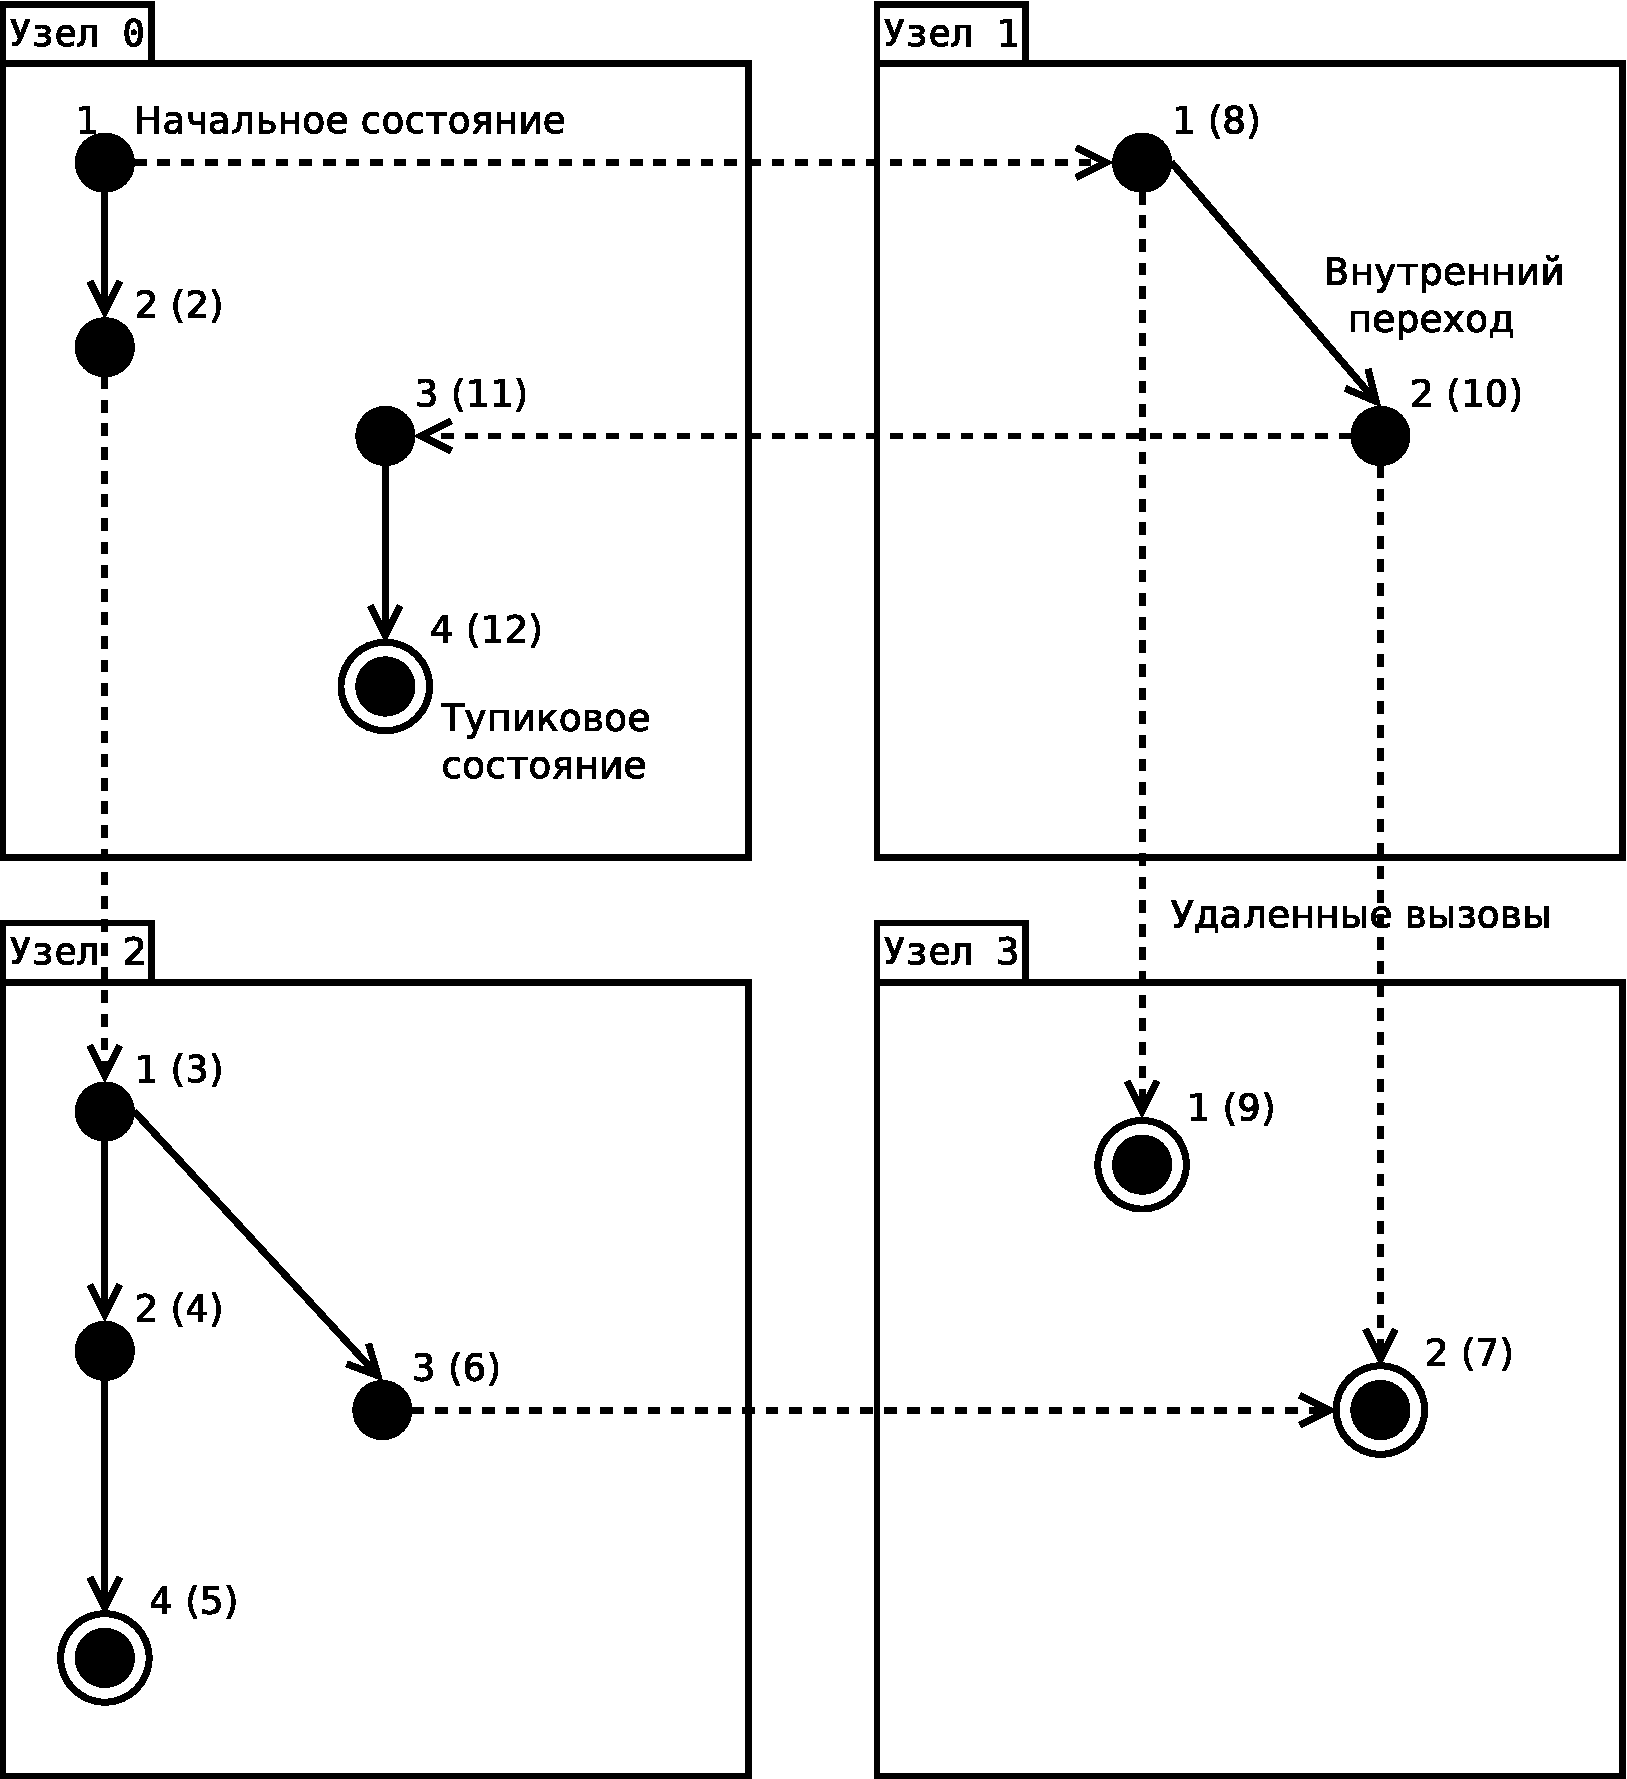
\includegraphics[height=0.85\textheight]{../graphics/distr-generation}
\end{minipage}
\begin{minipage}[m]{0.45\linewidth}
  \begin{flushleft}
    \begin{itemize}
    \item Используется вычислительная мощность всех узлов
    \item Удаленные вызовы асинхронные
    \item Можно уменьшить число удаленных вызовов
    \end{itemize}
  \end{flushleft}
\end{minipage}

\section{Предложенные способы распределения хранимых состояний между вычислительными узлами}
\label{sec:state-partitioning}

\begin{minipage}[m]{0.7\linewidth}
  \includegraphics[width=1\textwidth]{../graphics/state-partition-slides}  
\end{minipage}
\begin{minipage}[m]{0.3\linewidth}
  $$ M_1 = T \cdot (1 - \frac{1}{N}) $$
  \\ ~ \\
  $$ M_2 = \frac{T}{P} \cdot (1 - \frac{1}{N}) $$
\end{minipage}

\begin{center}
  $N$~--- число узлов, $T$~--- переходов между состояниями, \\
  $M$~--- сообщений между узлами
\end{center}

\section{Схема хранения состояний в ОЗУ узла}
\label{sec:state-store-full}

\begin{center}
  \includegraphics[width=0.9\textwidth]{../graphics/fullstate-slides}
\end{center}

\section{Компоненты разработанного ПО}
\label{sec:component-diag}

\begin{center}
  \includegraphics[width=1\textwidth]{../graphics/components}
\end{center}

\section{Компоненты параллельного генератора состояний}
\label{sec:component-diag}

\begin{center}
  \includegraphics[width=1\textwidth]{../graphics/stategen-components}
\end{center}

\section{Взаимодействие двух MPI-процессов}
\label{sec:mpi-sequence}

\begin{center}
  \includegraphics[height=0.88\textheight]{../graphics/mpi-async-seq}
\end{center}

\section{Трансляция описания модели в граф команд}
\label{sec:pmlparse}

\begin{minipage}[m]{0.35\linewidth}
  \begin{lstlisting}[language=Promela,style=simplecode,numbers=none]
    do
    :: x == 1 -> y = 2
    :: x == 2 -> y = 1
    :: else  -> break
    od;
    channel1 ! x,y
  \end{lstlisting}
\end{minipage}
\begin{minipage}[m]{0.75\linewidth}
  \includegraphics[height=0.85\textheight]{../graphics/pmlparse-inner}
\end{minipage}

\section{Исследование}
\label{sec:experim}

\begin{itemize}
\item Сравнение разработанного ПО с существующим
\item Сравнение методов распределения состояний
\end{itemize}

\begin{center}
  \includegraphics[width=1\textwidth]{../graphics/exp-idef0}
\end{center}

\section{Исходные данные для экспериментов}
\label{sec:experim-input}

\begin{minipage}[t]{0.15\linewidth}
Модели:  
\end{minipage}
\begin{minipage}[t]{0.85\linewidth}
  \begin{itemize}
  \item Обедающие философы, число сторон от 5 до 8
  \item Алгоритм выбора лидера, число сторон от 4 до 7
  \end{itemize}

\end{minipage}
\begin{center}
  \includegraphics[width=1\textwidth]{../graphics/mpi-deploy-horz}
\end{center}

\section{Зависимость требуемого времени от числа состояний}
\label{sec:states-time}

\begin{center}
  \includegraphics[height=0.88\textheight]{../data/plots/states-speed}
\end{center}

% \section{Сравнение скорости генерации состояний}
% \label{sec:stategen-speed}

% \begin{tabular}{ccccc}
%   \hline
%   Модель & Число     & ПО Spin,   & Разработанное ПО, & Отношение \\
%   & процессов & сост./сек &  сост./сек         & скоростей \\
%   \hline
%   Election & 6 & 1622583 & 2179986 & 1.3 \\
%   Peterson & 4 & 3940962 & 2082656 & 0.5 \\
%    & 5 & 2538418 & 2657356 & 1.0 \\
%   Philo & 5 & 3063200 & 1223386 & 0.4 \\
%    & 6 & 3080406 & 1893468 & 0.6 \\
%   \hline
% \end{tabular}

\section{Сравнение способов распределения состояний}
\label{sec:partition-cmp}

\begin{minipage}[m]{0.5\linewidth}
  \includegraphics[width=1.1\textwidth,page=1]{../data/plots/state-partition1-horz}  
\end{minipage}
\begin{minipage}[m]{0.5\linewidth}
  \includegraphics[width=1.1\textwidth,page=2]{../data/plots/state-partition1-horz}  
\end{minipage}

\small{
  \begin{minipage}[m]{0.5\linewidth}
    $$ \tau = \frac{\text{Суммарное число сообщений}}{\text{Суммарное число переходов}} $$    
  \end{minipage}
  \begin{minipage}[m]{0.5\linewidth}
    $$ \xi = \sigma_S/\overline{S}$$ $$ S_i - \text{число состояний на узле~} i $$
  \end{minipage}
}

\section{Выводы}
\label{sec:conclusion}

\small
\begin{enumerate}
\item Проанализированы проблемы проверки моделей и существующие подходы к их решению
\item Спроектирован и реализован алгоритм параллельной генерации состояний конечной
  модели
\item Предложен метод автоматического распределения состояний, уменьшающий число сообщений
  между узлами
\item Проведены эксперименты и проанализированы их результаты
\end{enumerate}

По результатам работы имеется одна публикация.

\end{document}

%%% Local Variables: 
%%% mode: latex
%%% TeX-master: t
%%% End: 
